\section{Unequal cells and a bound independent of their number}
\label{sec:cells}

The Fourier decomposition above requires identical cells. We now eliminate
the interiors of unequal cells directly, retaining every boundary degree
of freedom. This proves Theorem~\ref{thm:cells}.

Let the cell lengths be $h_i=8j_i+2$, $0\le i<r$, and write
$b_0=0$, $b_i=\sum_{a<i}h_a$, with all vertices interpreted modulo $N$.
For each cell retain the ordered six-tuple
\begin{equation}
 K_i=(b_i,b_i+1,b_i-4,b_i-3,b_i-2,b_i-1)
 \label{eq:retained}
\end{equation}
and eliminate its interior
\[
 I_i=\{b_i+2,\ldots,b_i+h_i-5\}.
\]
Thus $K_i$ contains the head pair of cell $i$ and the tail four vertices
of cell $i-1$. The $K_i$ and $I_i$ partition the vertices for every
legal $h_i\ge10$.

The range-four expansion \eqref{eq:two-walks} shows that different
interiors do not couple: adjacent interiors have closest separation seven.
Distinct retained intervals also have no direct coupling, since their
closest separation across cell $i$ is $h_i-5\ge5$.
Each interior is a chain of $2j_i-1$ four-site blocks; it couples only
to $K_i$ at its left and the tail-four slot of $K_{i+1}$ at its right.
The common initial and terminal triangle signs make these endpoint
coefficients independent of the cell length.

In terms of \eqref{eq:boundary-data}, the intrinsic retained block and
left and right chain couplings are
\begin{equation}
 \mathcal B=\begin{pmatrix}G_0&C_0\\C_0^T&D_c\end{pmatrix},
 \qquad U_0=\begin{pmatrix}R_0\\W_0^T\end{pmatrix},
 \qquad V=\begin{pmatrix}0_{4\times2}&E_+\end{pmatrix}.
 \label{eq:assembly-data}
\end{equation}
The global seam initially multiplies $C_0$ and the lower part of $U_0$
in $K_0$ by $\alpha$. Conjugating the tail-four coordinates of $K_0$ by
$\alpha$ restores \eqref{eq:assembly-data} and moves the seam sign to the
last chain's terminal coupling. Hence the canonical terminal factors are
\[
 \omega_i=1\quad(i<r-1),\qquad\omega_{r-1}=\alpha.
\]
This is an explicit permutation and diagonal sign conjugacy.
\begin{figure}[tbp]
\centering
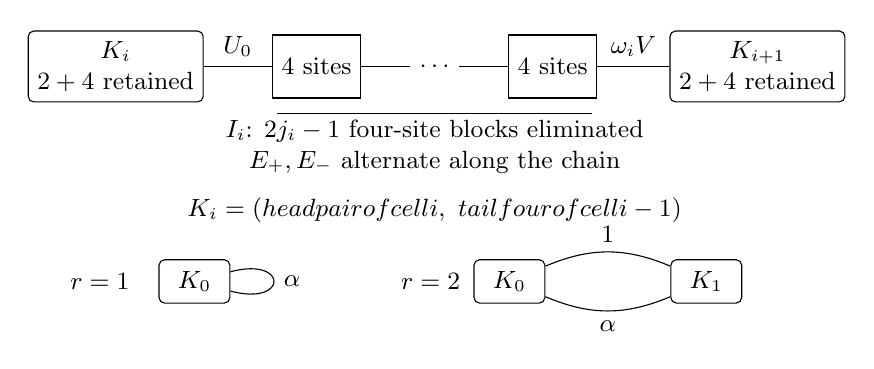
\begin{tikzpicture}[x=1cm,y=1cm,font=\small,
 core/.style={draw,rounded corners=2pt,minimum width=1.55cm,minimum height=.9cm,align=center},
 block/.style={draw,minimum width=1cm,minimum height=.8cm,align=center}]
\node[core] (kl) at (0,0) {$K_i$\\$2+4$ retained};
\node[block] (a) at (2.55,0) {$4$ sites};
\node (dots) at (4.05,0) {$\cdots$};
\node[block] (b) at (5.55,0) {$4$ sites};
\node[core] (kr) at (8.15,0) {$K_{i+1}$\\$2+4$ retained};
\draw (kl)--node[above] {$U_0$}(a);
\draw (a)--(dots); \draw (dots)--(b);
\draw (b)--node[above] {$\omega_i V$}(kr);
\draw (2.05,-.6)--(6.05,-.6);
\node[align=center] at (4.05,-1.02)
 {$I_i$: $2j_i-1$ four-site blocks eliminated\\$E_+,E_-$ alternate along the chain};
\node[align=center] at (4.05,-1.83)
 {$K_i=(\text{head pair of cell }i,\ \text{tail four of cell }i-1)$};
\node at (-.2,-2.73) {$r=1$};
\node[core,minimum width=.9cm,minimum height=.55cm] (one) at (1,-2.73) {$K_0$};
\draw (one) edge[loop right,looseness=8] node[right] {$\alpha$} (one);
\node at (4,-2.73) {$r=2$};
\node[core,minimum width=.9cm,minimum height=.55cm] (twoa) at (5,-2.73) {$K_0$};
\node[core,minimum width=.9cm,minimum height=.55cm] (twob) at (7.5,-2.73) {$K_1$};
\draw (twoa) to[bend left=23] node[above] {$1$} (twob);
\draw (twoa) to[bend right=23] node[below] {$\alpha$} (twob);
\end{tikzpicture}
\caption{Block couplings in $cI-A^2$, rather than individual graph edges.
The upper panel shows one interior chain when $j_i\ge2$; for $j_i=1$
it consists of one four-site block. The right coupling meets only the
tail-four slot of $K_{i+1}$. Eliminating all chains gives a cyclic matrix
on the $K_i$, with $\omega_i=1$ except $\omega_{r-1}=\alpha$.
The lower panels show the endpoint incidences when the cycle is a loop or
a pair of parallel chains: both contributions are added, and every core
has two incidences.}
\label{fig:boundary}
\end{figure}


\subsection{The additive cyclic Schur identity}

Use the same open pivot sequence as before and put
\[
 U_{a+1}=-U_aX_a^{-1}E_a.
\]
Equation~\eqref{eq:recurrence} gives $U_a=(R_a^T,W_a)^T$,
that is, the vertical stack of $R_a$ and $W_a^T$.
For the final interior index $p_i=2j_i-2$, define
\begin{equation}
 \mathcal L_i=\sum_{a=0}^{p_i}U_aX_a^{-1}U_a^T,
 \qquad \mathcal P_i=V^TX_{p_i}^{-1}V,
 \qquad F_i=U_{p_i}X_{p_i}^{-1}V.
 \label{eq:endpoint-data}
\end{equation}
Let $\iota_i:\R^6\to\R^{6r}$ be the coordinate embedding at $K_i$,
with the index $i+1$ understood cyclically.

\begin{lemma}[Exact cell assembly]\label{lem:assembly}
When the interior pivots are positive, their elimination gives the retained
matrix
\begin{align}
 \mathcal S={}&I_r\otimes\mathcal B
 -\sum_i\iota_i\mathcal L_i\iota_i^T
 -\sum_i\iota_{i+1}\mathcal P_i\iota_{i+1}^T\notag\\
 &-\sum_i\omega_i\bigl(
 \iota_iF_i\iota_{i+1}^T+\iota_{i+1}F_i^T\iota_i^T\bigr).
 \label{eq:assembly}
\end{align}
Every contribution is added, including coincident block locations when
$r=1$ or $r=2$.
\end{lemma}
\begin{proof}
At the current pivot of a chain, the left coupling is $U_a$, so the Schur
complement subtracts $U_aX_a^{-1}U_a^T$ from its retained left endpoint
and propagates the response as $-U_aX_a^{-1}E_a$.
Only the final pivot also sees the right endpoint, through $\omega_iV$.
Its two self-energy terms and cross term are precisely
\eqref{eq:endpoint-data}. Distinct interiors do not couple, so their
Schur contributions add.
For $r=2$, two different chains connect the same pair of retained cores;
both cross contributions remain in \eqref{eq:assembly}.
For $r=1$, the combined coupling at the final pivot is
$U_{p_0}+\omega_0V^T$. Expanding its quadratic Schur correction gives
$\mathcal P_0$ and the loop contribution
$\omega_0(F_0+F_0^T)$ in addition to $\mathcal L_0$.
Thus the same additive formula also covers the one-cell case.
\end{proof}

\subsection{The common limit and the degree-two estimate}

At either certified cap, suppose $p_i=J+2s_i$ with $s_i\ge0$, and put
$s=\min_i s_i$. Define
\[
 \mathcal L_\infty=\sum_{a\ge0}U_aX_a^{-1}U_a^T,
 \qquad \mathcal P_\infty=V^TX_*^{-1}V.
\]
By the stacked form of $U_a$, the matrix
$\mathcal B-\mathcal L_\infty-\mathcal P_\infty$ equals exactly
$S_\infty$ from \eqref{eq:Sinfty}. Its positivity has already been
proved; there is no new limiting-core assumption.

The separate response bounds give
\[
 \norm{U_{J+2v}}_2\le\sqrt2\,a q^v,
 \qquad \norm{U_{J+2v+1}}_2\le\sqrt2\,b q^v.
\]
Counting both increments in every pair therefore yields
\begin{equation}
 \norm{\mathcal L_\infty-\mathcal L_i}_2
 \le\frac{12b^2q^{2s_i}}{1-q^2}.
 \label{eq:Ltail}
\end{equation}
The right side harmlessly includes the final included term as well as
the actual suffix. The inverse identity and $\norm V_2\le\sqrt{14}$
give
\begin{equation}
 \norm{\mathcal P_i-\mathcal P_\infty}_2
 \le576\delta\theta^{s_i}.
 \label{eq:Ptail}
\end{equation}
Finally,
\begin{equation}
 \norm{F_i}_2\le3\sqrt{28}\,a q^{s_i}<16a q^{s_i}.
 \label{eq:Ftail}
\end{equation}

The diagonal part of \eqref{eq:assembly}, relative to
$I_r\otimes S_\infty$, combines one outgoing error from
\eqref{eq:Ltail} with one incoming error from \eqref{eq:Ptail}.
For the cross terms, take arbitrary $v_i\in\R^6$. Their quadratic form
has absolute value at most
\begin{align*}
 \sum_i2\norm{F_i}_2\norm{v_i}_2\norm{v_{i+1}}_2
 &\le\sum_i\norm{F_i}_2(\norm{v_i}_2^2+\norm{v_{i+1}}_2^2)\\
 &\le2\max_i\norm{F_i}_2\sum_i\norm{v_i}_2^2.
\end{align*}
Each retained core has exactly two chain-end incidences, counting a loop
twice and retaining both parallel contributions. This proves the bound
for every $r\ge1$, without summing an error $r$ times. We obtain
\begin{equation}
 \norm{\mathcal S-I_r\otimes S_\infty}_2
 \le E_s:=\frac{12b^2q^{2s}}{1-q^2}
              +576\delta\theta^s+32a q^s.
 \label{eq:assembly-error}
\end{equation}

\begin{proof}[Proof of Theorem~\ref{thm:cells}]
Exact arithmetic with the two parameter columns gives
\[
 E_0=
 \begin{cases}
 501647/468750000<1/500,&c=\czero,\\
 700000123/196875000000000000<10^{-8},&c=\cone.
 \end{cases}
\]
All terms in $E_s$ decrease with $s$. Proposition~\ref{prop:tail} already
supplies $S_\infty\succ(\gamma-\epsilon)I_6$, so
\eqref{eq:assembly-error} gives
\[
 \mathcal S\succ(\gamma-2\epsilon)I_{6r}\succ0.
\]
The condition $p_i=2j_i-2\ge J$ is exactly
$h_i\ge4(J+2)+2$, namely $106$ or $202$. All eliminated pivots are
positive by Section~\ref{sec:uniform}. Schur congruence now proves
$cI-A_N(\tau,\alpha)^2\succ0$, as required.
\end{proof}

The reduction is now uniform in both sources of variation: the shortest
cell controls the local tail, and two chain-end incidences at each retained
core control the global error. The full boundary matrix therefore remains
positive as the number of legal cells increases.
